\chapter{Algoritmos de Segmentação}\label{cap:algoritmos}

Este capítulo descreve 4 técnicas de segmentação de imagens, sendo a por limiar (\textit{thresholding}) a mais simples. As técnicas baseadas em bordas e regiões são mais complexas e demandam um ônus computacional mais elevado.

% \section{Tipos de Algoritmos}
\begin{itemize}
    \item \textit{Thresholding};
    \item Método Baseado em Bordas; e  
    \item Método Baseado em Regiões
    \begin{itemize}  
        \item \textit{Split and Merge}; e
        \item \textit{Watershed}.
    \end{itemize}
\end{itemize}

\subsection{\textit{Thresholding}}\label{sec:alg_thresholding}
É um método simples de segmentação de imagens.
Busca dividir a imagem em duas categorias: objetos (\textit{foreground}) e plano de fundo (\textit{background}). 
Cada \textit{pixel} é alocado a uma categoria de acordo com seu valor em níveis de cinza.

Dado um limiar T (\textit{threshold}), o \textit{pixel} com valor $f_i_j$  e localizado na posição (i,j)  é alocado à:
\\
\begin{cases}
$  categoria 1, se: f_{ij} $\leq$ T. $ \\
$  categoria 2, caso contrário. $ \\
\end{cases}
\\
O limiar T pode ser escolhido manualmente, tentando diferentes valores de T e analisando qual deles é mais eficiente na identificação dos objetos de interesse.
O \textit{threshold} T também pode ser escolhido a partir do histograma da imagem, e escolhe-se T como o valor entre as duas distribuições de cinza.

A seguir há a figura \ref{fig:einstein}, uma imagem original do Einstein,  e as duas formas de segmentação de imagens por limiar (\textit{thresholding}). Enquanto na figura \ref{fig:einsteinglobal} há um limiar T fixo , na  figura \ref{fig:einsteinlocal} ele é variável.

\subsection*{\textit{Threshold} Global}
O mesmo valor de T é usado para a imagem inteira.

% Figura 
  \begin{figure}[!htb]
       \begin{center}  
          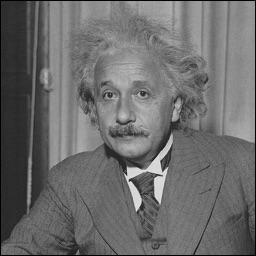
\includegraphics[width=0.3\columnwidth]{img/einstein.jpg}
           \caption{\label{fig:einstein}Imagem original\citep{stanford}.}
           % \vspace{2.0em}
       \end{center}
   \end{figure}

% Figura 
  \begin{figure}[!htb]
       \begin{center}  
          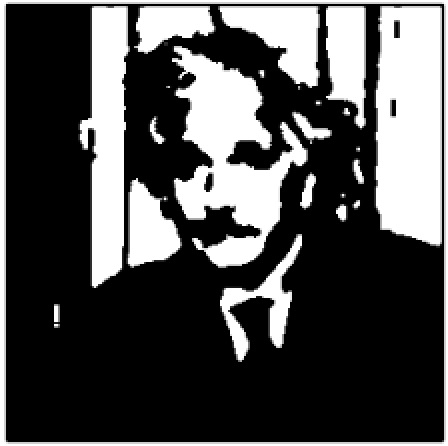
\includegraphics[width=0.3\columnwidth]{img/einstein-globalthresholding127.jpg}
           \caption{\label{fig:einsteinglobal}Imagem segmentada pelo algoritmo threshold global.}
           % \vspace{2.0em}
       \end{center}
   \end{figure}

\subsection*{\textit{Threshold} Local (ou dinâmico)}
Divide-se a imagem em regiões distintas e adota-se um valor T para cada uma delas, onde esse valor funcionará como threshold local. 

% Figura 
  \begin{figure}[!htb]
       \begin{center}  
          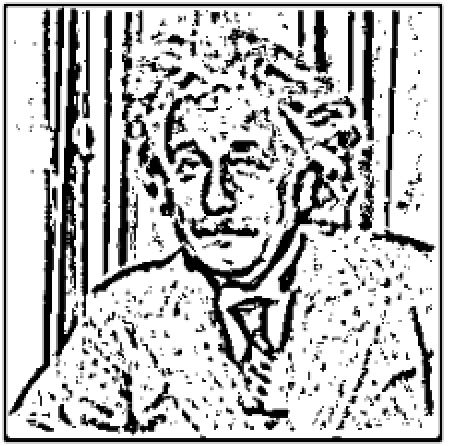
\includegraphics[width=0.3\columnwidth]{img/einstein-localthresholding-adaptivegausian.jpg}
           \caption{\label{fig:einsteinlocal}Imagem segmentada pelo método de segmentação thresholding local, chamado de adaptive gaussian  thresholding.}
           % \vspace{2.0em}
       \end{center}
   \end{figure}
   
   Pode-se observar pela figura \ref{fig:einsteinlocal} que houve a separação em mais regiões nesse método do que na figura \ref{fig:einsteinglobal}, já que foi usado um limiar mais apropriado a cada região.

\subsection{Baseado em Bordas}
Primeiramente, classifica-se os \textit{pixels} como “borda” ou “não-borda”.
Depois, divide-se a imagem em regiões, baseado nas bordas detectadas.

As bordas são identificadas por meio das descontinuidades, isto é, variações abruptas nos valores dos \textit{pixels}. 

Como pode-se perceber na figura \ref{fig:smandrill}, por esse método houve a segmentação da imagem de um macaco em regiões de olhos, nariz e outras partes. 

% ------------------------------------------------------------------------------------------------------------
% Figura 
\begin{figure}[!htb]
 \centering
 \def\baselinestretch{1}\small\normalsize
 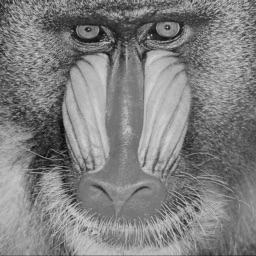
\includegraphics[width=0.4\textwidth]{img/stf-smandrill.jpg}\qquad
 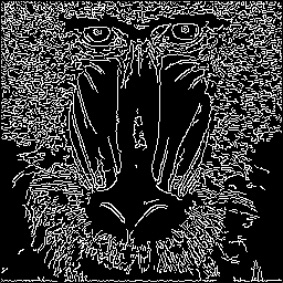
\includegraphics[width=0.4\textwidth]{img/stf-smandrill-edgedetect.jpg} 
 \caption{\label{fig:smandrill} Uma imagem de um macaco \citep{stanford} à esquerda e à direita segmentada pelo método de detecção de bordas em linguagem de programação python.}
 %\vspace{2.0em}
\end{figure}


\subsection{Baseado em Regiões}
\subsubsection*{O que é uma região?}
Uma região pode ser “definida” como um grupo de \textit{pixels} conectados com propriedades similares.

Porém, é um conceito importante e difícil de definir, já que depende da interpretação do que seria uma região  em determinado caso.

Pelas figuras da seção \ref{sec:segmenthm} do capítulo \ref{cap:segmentacao}, nota-se as diferentes interpretações do conceito de região pelas diferentes quantidades de regiões notadas por humanos nas Figuras \ref{fig:Berkeley_mulher_segmentada} e \ref{fig:Berkeley_mulher_segmentada2}. Tal fato também acontece com os computadores, como nota-se pelas figuras \ref{fig:indiosegmentado}.

\subsubsection{\textit{Split and Merge}}
\subsubsection*{Procedimento}
As etapas fundamentais deste algoritmo segundo  são: 
\begin{enumerate}
    \item Criar critério para definir o que é uma área homogênea.
    \item Começar com a imagem completa e divide em 4 sub-imagens.
    \item Checar cada sub-imagem e dividi-la novamente em 4 novas sub-imagens caso ela não seja homogênea.
    \item Repetir Passo 3 até que não se consiga mais subdividir.
    \item Comparar sub-imagens com suas regiões vizinhas e agrupá-las se forem homogêneas.
    \item Repetir Passo 5 até que não se consiga mais agrupar.
\end{enumerate}

\subsubsection*{EXEMPLO - \textit{QUADTREE}}
Um exemplo de segmentação baseada em região Split and Merge é o algoritmo quadtree. A figura \ref{fig:aral} abaixo ilustra a segmentação de imagem por este algoritmo, e observa-se a segmentação da região que contém água na figura.

% ------------------------------------------------------------------------------------------------------------
% Figura 
\begin{figure}[!htb]
 \centering
 \def\baselinestretch{1}\small\normalsize
 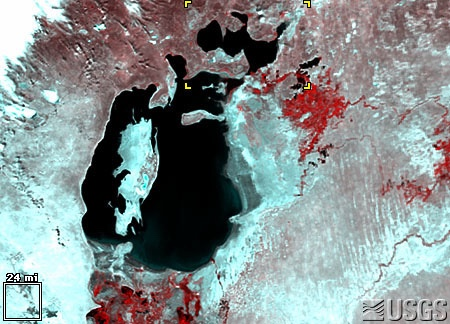
\includegraphics[width=0.4\textwidth]{img/stf-aral1997.jpg}\qquad
 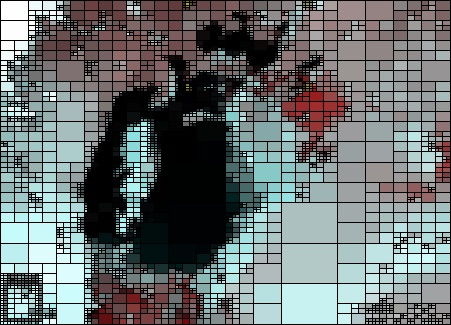
\includegraphics[width=0.4\textwidth]{img/stf-aral1997-quadtree.jpg} 
 \caption{\label{fig:aral}Uma representação visual de uma região \citep{stanford} à esquerda e à direita segmentada pelo algoritmo quadtree em linguagem de programação python.}
 %\vspace{2.0em}
\end{figure}

\subsubsection{\textit{Region growing} (abordagem \textit{bottom-up})}
\subsubsection*{Procedimento}
As etapas fundamentais deste algoritmo são: 
\begin{enumerate}
    \item Identificar o ponto de partida.
    \item Incluir \textit{pixels} vizinhos com características similares (nível de cinza, textura, cor, etc).
    \item Continuar até que todos os \textit{pixels} estejam associados com um dos pontos de partida.
\end{enumerate}

\subsubsection*{EXEMPLO - \textit{WATERSHED}}
Um exemplo de segmentação baseada no método \textit{Region growing} é o algoritmo \textit{watershed}. A figura \ref{fig:coins} abaixo ilustra a segmentação de imagem por este algoritmo, e observa-se regiões distintas correspondentes à cada moeda da figura.

% ------------------------------------------------------------------------------------------------------------
% Figura 
\begin{figure}[!htb]
 \centering
 \def\baselinestretch{1}\small\normalsize
 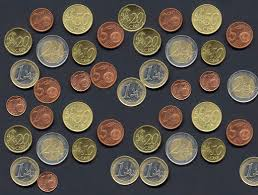
\includegraphics[width=0.4\textwidth]{img/stf-coins.jpg}\qquad
 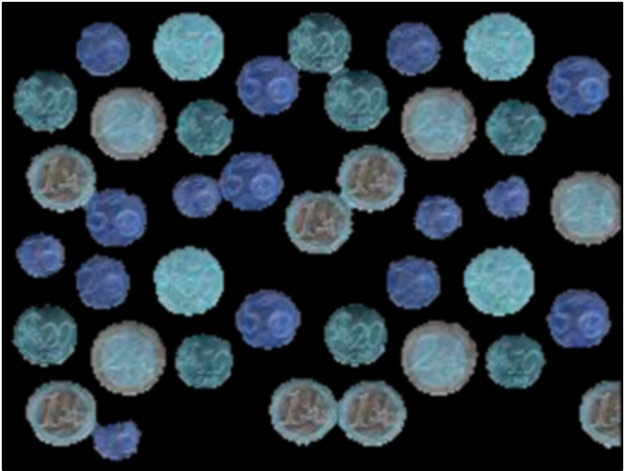
\includegraphics[width=0.4\textwidth]{img/stf-coins-watersheed.jpg} 
 \caption{\label{fig:coins}Imagem de uma moeda \citep{stanford} à esquerda e à direita segmentada pelo algoritmo watersheed em linguagem de programação python.}
 %\vspace{2.0em}
\end{figure}
 
% Stanford DataSet
%  https://scien.stanford.edu/index.php/test-images-and-videos/
 

